\section{Dataset}

\begin{frame}{About Dataset}

  \begin{itemize}
    \item The Breast Cancer Wisconsin (Diagnostic) Data Set
    \item 569 rows with 33 attributes
    \item Features are computed from a digitized image of a fine needle aspirate (FNA) of a breast mass.
    \item Describe characteristics of the cell nuclei present in the image
  \end{itemize}
  
\end{frame}

\begin{frame}{Parameter of Interest}

  \begin{itemize}
    \item perimeter\_mean
    \item the mean size of the core tumour
  \end{itemize}

  \vspace{0.25in}

  \begin{figure}
    \centering
    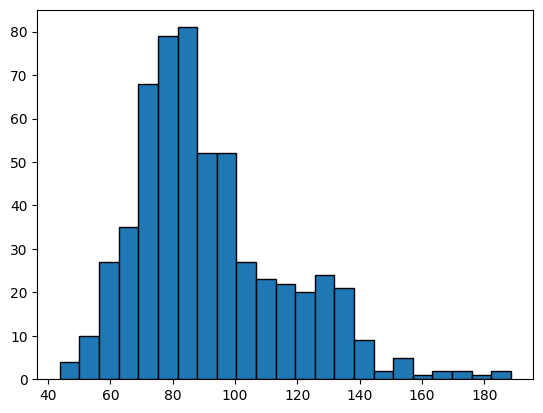
\includegraphics[width=0.5\linewidth]{../Report/images/data-hist.png}
    \caption{Histogram of Perimeter Mean}
  \end{figure}
  
\end{frame}
